\chapter{Implementation}
This chapter deals with the implementation-specific details, in which programming paradigms, algorithms, and architectures used will be discussed. Specifically the chapter will discuss how the pre-processing is implemented in an object-oriented, imperative fashion, how features are extracted from the pre-processing features, and how this is achieved in a continuous fashion, on the device.


\section{Pre-processing}
As previously mentioned, the goal of the pre-processing step is to reduce the raw dataset to a more condensed representation such that subsequent algorithms will have fewer data points to process, and thus run faster and consume less energy. The reason why it is possible to save compute power by doing this, is because the DBSCAN algorithm used for finding places does not take the time dimension into account. By simply running through the data points in temporal ordering, it is possible to group points into so called Stops, which represent a temporal, and small-scale distance clustering of raw points, which are then used in the DBSCAN algorithm to identify significant places. In addition, Moves are also computed between stops, such that movement-related features can be calculated, such as distance travelled. The original implementation of these pre-processing algorithms were implemented in Python by Jonas Busk, which used vectorized computations, which Dart does not support nearly to the same extent. The algorithms therefore had to be changed slightly, and were re-implemented using a functional programming approach wherever applicable. For certain computations a more traditional imperative approach, using for-loops, was utilized.

\subsection{Finding Stops}
Firstly the raw data points are clustered based on their time-ordering and distance from each other. By reducing the raw data points to more coarse grained stops, the will become easier for identifying significant places, which is can be done since the time-ordering of the data points tell us which points can belong together in a stop. This is done by iterating over the ordered data points and building a cluster from these data points, recalculating the cluster centroids with each added data point. This is repeated until the current data point is too far away from the cluster centroid and the cluster is then saved as a stop, and a new cluster is built from the current data point. This process is repeated until all data points have been considered, which means all data points will belong to exactly one stop, and that each stop contains at least one raw data point. The parameter for finding stops is the \verb|MOVE_DIST|, i.e. the radius of each stop-cluster. The lower the parameter value, the more clusters will be found. Each stop has an assigned place, however at this stage we have not yet identified the significant places and for that reasons we assign the null-place to each stop, and assign the place later.

\begin{minted}{python}
def find_stops(dataset):
    stops = []
    n = dataset.length
    for i = 0 to n:
        j = i + 1
        cluster = dataset[i:j]
        
        # Expand stop-cluster
        while dist(cluster.centroid, dataset[j]) <= MOVE_DIST and j < n:
            j += 1
            cluster = dataset[i:j]
        
        # Current data point data[j] is outside the cluster 
        l = Location(cluster.centroid.lat, cluster.centroid.lon)

        # Create unlabelled stop with place ID -1
        s = Stop(l, cluster.arrival.min, cluster.departure.max, -1) 
        stops.add(s)
        
        # Move beyond already-seen data points
        i = j
    return stops
\end{minted}


\subsubsection{Significant Places}
For finding the significant places the stops are clustered with the DBSCAN algorithm, which will use a density-based approach to finding clusters. The parameter \verb|PLACE_DIST| is used as the max-distance between points used by DBSCAN and the Haversine distance function. The DBSCAN algorithm will assign each stop given as input with a label, which is a non-negative number for all significant places and $-1$ for all noisy stops signifying the null-place, i.e. stops not belonging to a place. After this, each stop have now been assigned a place they belong to, and this is set explicitly such that time spent at a place can be counted later.

\begin{minted}{python}
def find_places(stops):
    places = []
    
    # Perform DBSCAN clustering on stops
    labels = DBSCAN(stops, PLACE_DIST)
    
    # Aggregate stops on their assigned label
    groups = stops.group_by(labels)
    
    for id, group in (labels, groups)
        l = Location(group.lat.median, g.lon.median)
        p = Place(id, l)
        places.add(p)
        
        # Assign the current place id to each stop in the group
        for s in group:
            s.placeId = id
    
    return places, stops
\end{minted}

\subsubsection{Moves}
The moves made by the user is found by iterating over each stop and assigning all the data points which were visiting between each pair of stops, i.e. $s_i$ and $s_{i + 1}$ to it, as well as the two stops. Through this, the distance of the point-chain can be calculated, as well as the duration of the transition-period.

\begin{minted}{python}
def find_moves(dataset, stops):
    moves = []
    
    # Find all data points between each pair of stops
    for i = 0 to stops.length
        cur = stops[i]
        next = stops[i+1]
        points = dataset.filter(cur.departure <= d.timestamp 
            and d.timestamp <= next.arrival)
        m = Move(cur, next, points)
    
    return moves
\end{minted}

\subsection{Distance Function}
Geodesic vs Haversine discussion here
For all distance measures, the Haversine distance function was used due to being far easier to compute and implement and provides the same results for shorter distances, which is the case for the processing in this context. This also saves battery life. 


\begin{minted}{python}
collect_data_continuously()
on data_point:
	save_to_disk(data_point)
	if trigger:
        points = load_todays_data_from_disk()
		stops_hist, moves_hist = load_from_disk()
		stops = stops_hist + find_stops(points)
		moves = moves_hist + find_moves(stops, points)
		features = feature_extraction(stops, places, moves)
		# do something with the features
		save_to_disk(stops, moves)
\end{minted}

\subsection{Feature Extraction}
The feature extraction takes place after the data collection and pre-processing has been done, and will use the Stops, Places and Moves to derive the features described in Chapter ??. 

\subsubsection{Number of Clusters}
Defined as the number of non-negative place labels found by the Places algorithm.

\begin{minted}{python}
def num_clusters(places):
    return len(places > 0)
\end{minted}

\subsubsection{Location Variance (LV)} 
LV was computed as the natural logarithm of the sum of the statistical variances of the latitude and the longitude components of the location data. The dataset must contain at least 2 observations to calculate the variance, otherwise the variance of both the latitude- and the longitude will be zero, and thus $LV = log(0 + 0 + 1)  = 0$

\begin{minted}{python}
def location_variance(dataset):
    return log(var(dataset.lat) + var(dataset.lon.var) + 1)
\end{minted}

\subsubsection{Location Entropy (LE)} 
Here, we use the duration spent at each place, found in the duration column in the places dataframe.

\begin{minted}{python}
def entropy(places):
    p = places.duration / sum(places.duration)
    return -sum(p * log(p))
\end{minted}

\subsubsection{Normalized LE} 
Here we just divide LE by the log to the number of places.

\begin{minted}{python}
def normalized_entropy(places):
    return entropy(places) / log(places.length)
\end{minted}

\subsubsection{Time-distribution Table}
The time distribution table tells the story of which places were visited for how long during the day and does this by dividing the day into 24 one-hour time slots represented by rows, and the columns representing the different significant places found by the pre-processing algorithms. Each entry $T[i,j]$ is the number of hours spent at timeslot $i$ at place $j$, which means that the row can maximally sum to 1.0. If the user moves between two places, the row will however not sum to 1.0 since there was time spent at none of the places.

Using the stops, the time spent at each place can be calculated for each hourly timeslot during the day. Concretely, this is done by iterating through each stop and incrementing the time at entry $i,j$ using the arrival time of the stop \verb|1 - row.arrival.minute / 60| by using the \verb|arrival.hour| as the hour slot. For the last time slot the same is done, but using the departure time \verb|row.departure.minute / 60|. Every time slot in between for the the place $j$ is set to 1.0 since the user was there for the full time slot.

\begin{minted}{python}
def make_hour_matrix(stops, num_places):
    h = np.zeros((HOURS_IN_A_DAY, num_places))
    
    for index, row in stops.iterrows():
        pid = row.place
        start_hour = row.arrival.hour
        end_hour   = row.departure.hour
        
        # If user arrived and departed within the same hour
        # Then the time stayed is the diff between departure and arrival
        if start_hour == end_hour:
            h[start_hour, pid] = row.departure.minute - row.arrival.minute
        
        else:
            # Arrival hour
            h[start_hour, pid] = 60 - row.arrival.minute

            # In between
            for hour in range(start_hour+1, end_hour):
                h[hour, pid] = 60

            # Departure hour
            h[end_hour, pid] = row.departure.minute
        
    return h / 60 # Normalize by 60 mins
\end{minted}

\begin{figure}
    \centering
    \begin{tabular}{|l|l|l|l|l|}
    \hline
    \textbf{}        & \textbf{Place \#0} & \textbf{Place \#1} & \textbf{...} & \textbf{Place \#n} \\ \hline
    \textbf{00 - 01} &                    &                    &              &                    \\ \hline
    \textbf{01 - 02} &                    &                    &              &                    \\ \hline
    \textbf{...}     &                    &                    &              &                    \\ \hline
    \textbf{16 - 17} &                    &                    &              &                    \\ \hline
    \textbf{17 - 18} &                    &                    &              &                    \\ \hline
    \textbf{18 - 19} &                    &                    &              &                    \\ \hline
    \textbf{...}     &                    &                    &              &                    \\ \hline
    \textbf{23 - 00} &                    &                    &              &                    \\ \hline
    \end{tabular}
    \caption{Time-place distribution table.}
    \label{fig:time-table}
\end{figure}

\subsubsection{Home Stay} 
The percentage of time the participant has been home place, home being the most visited cluster between 12 am and 6 am which can be identified by using the mean of the the historical time distribution tables, i.e. the place which, on average, was the most visited between 00 and 06 am. Afterwards, all the stops during the day are iterated and the duration of the stops belonging to the home cluster are summed up.

\subsubsection{Transition Time} 
To calculate the transition time of the user the Moves are used, and the difference is time stamps between all the individual data points which make up each move are summed together. 

\subsubsection{Total Distance} 
Same procedure as transition time, except for using the the distances between all the individual data points rather than the duration.

\subsubsection{Routine Index} 
The Routine Index is the RMSE of today's time distribution table compared the historical table, which is the average of all historical tables. The historical tables are computed by loading all historical stops from the disk, and calculating the tables from these. The routine index is always calculated based on the current hour of the day, i.e. at 14:00 only the time-slots from 00:00 to 14:00 are compared to the historical average, between 00:00 and 14:00. 

\begin{minted}{python}
def RI(m, h, end_hour=24):
    if m.sum() == 0:
        # no routine index could be calculated
        return -1.0 
    return 1 - np.abs(m[:end_hour] - h[:end_hour]).mean()
\end{minted}

\begin{figure}
    \centering
    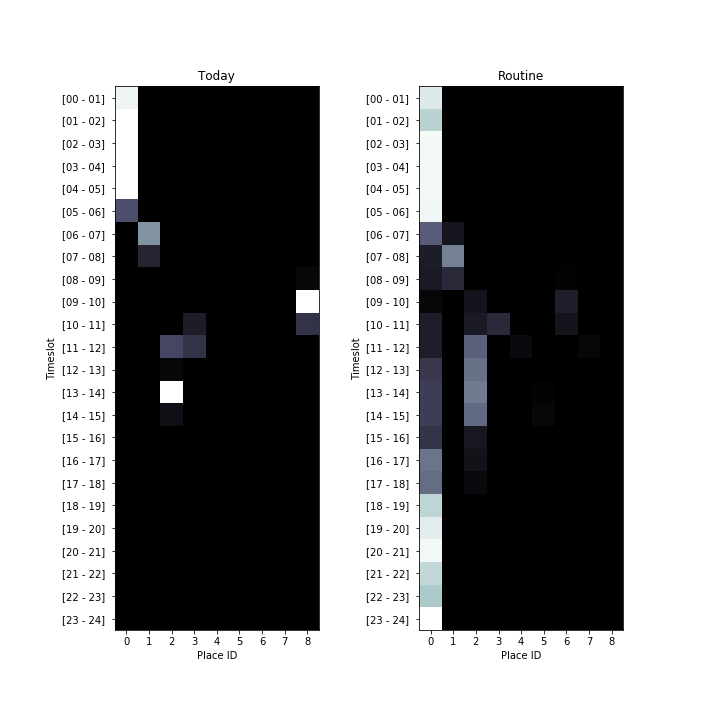
\includegraphics[width=\textwidth]{images/routine.png}
    \caption{An hour matrix of a specific day compared to the Routine Matrix derived from several days of data.}
    \label{fig:routine_example}
\end{figure}

\section{Storing Objects on the Device}
It was necessary to store Stops and Moves on the device, such that which rely on historic data can be computed in the future. For a single day it is also necessary to store all the data points collected on that day, on the disk, in order to minimize the risk of data loss. This was done by defining a buffer of data points which collects all incoming GPS data, and once a certain capacity is reached the data contained in the buffer is written to the disk, and the buffer is emptied.

\subsection{Serialization}
In order to save the SingleLocationPoints from today and historical Stops and Moves on the device they must be transformed from Dart objects into a data format which can store the state of the object, i.e. the information contained within it. The process of doing so is serialization and in this case Dart objects were transformed into JavaScript Object Notation (JSON) objects, which is a very common, human-readable data format that uses key-value pairs to store data. A JSON object can be stored in a database, or it can be transformed to a string in order to be stored. It was chosen to simply transform JSON objects to a string and write them to a local file, rather than storing the information in a database on the phone. The database approach is more involved and was therefore not chosen given the small scope of the project and working from a philosophy of getting a prototype up and running as fast as possible.

JSON supports a limited number of data types, such as strings, numbers, booleans, arrays, objects and null values. This means that in order to translate a Dart object to JSON, all of its fields must be serializable. An example of where this quickly becomes a problem, is with objects such as DateTime objects, since they are not supported by JSON - however a DateTime can be transformed to a number, which is milliseconds since epoch, or to an ISO standard date string. The approach is therefore to look at all the fields of the object that is to be serialized, and ensure that types of these fields all support some form of serialization. If they do not, it must be implemented.

\begin{figure}
    \centering
\begin{minted}{json}
{
    "location": {
        "latitude": 55.11787166161895,
        "longitude": 14.703046919371356
        },
    "datetime": "1586527196999"
}
\end{minted}
    \caption{Example of a serialized SingleLocationDataPoint}
    \label{fig:serialized_point}
\end{figure}

\begin{figure}
    \centering
\begin{minted}{json}
{
    "centroid": {
        "latitude": 55.11787908183754,
        "longitude": 14.703028176721789
        },
    "place_id": 0,
    "arrival": 1586556000999,
    "departure": 1586556697999
}
\end{minted}
    \caption{Example of a serialized Stop}
    \label{fig:serialized_stop}
\end{figure}

\begin{figure}
    \centering
\begin{minted}{json}
{
    "stop_from": {
        "centroid": {
            "latitude": 55.11053332998761,
            "longitude": 14.712282829580444
            },
        "place_id": 6,
        "arrival": 1586694154999,
        "departure": 1586696052001
    },
    "stop_to": {
        "centroid": {
            "latitude": 55.11793063393585,
            "longitude": 14.702982994031046
        },
        "place_id": 0,
        "arrival": 1586697230006,
        "departure": 1586699246824
    },
    "distance":2357.3408321427805
}
\end{minted}
    \caption{Example of a serialized Move}
    \label{fig:serialized_move}
\end{figure}


For loading an object from disk into application memory again it must also support de-serialization which reads values of the JSON object's keys and stores them in a Dart object. If we continue the example of a DateTime object which was serialized by either converting it to a number or a string, de-serialization must use a parser which reads the string bit by bit or use some math for calculating what day a time delta from January 1st 1970 is. 

Serialization and de-serialization is implemented by making an abstract class called Serializable, which has two functions: toJson and fromJson. The toJson function converts the object itself to a JSON object and the fromJson function is a so-called factory function which is in essence a constructor which creates a Dart object given a JSON object. The SingleLocationPoint, Stop and Move classes all implement the Serializable interface, which requires the classes to have a concrete implementation of these two methods, which in turn ensures the compiler that all of these classes can be serialized and de-serialized, which makes generalizing about objects belonging to either of these classes easier. Concretely, a generic class, Serializer<E>, was implemented in order to handle serialization, in which a type E is specified, which must a Serializable class. This makes it efficient in terms of lines of code to serialize a list of objects, since they are all required to implement toJson method, which produces a JSON object, and for de-serialization purposes they can all be constructed from a JSON object, given that it contains a set of correctly formatted key-value pairs.


\section{Unit Testing}
Mostly the model as well as read/writes to local files i.e. Serialization. 
\section{Tuning Parameters}
Parameter tuning was done by taking a few different examples where ground truth is  known, i.e. by having done it myself. The examples include whole days in Munich (GER), Copenhagen (DK) and Bornholm (DK) which all have vastly different environments and acitivties, with Munich having places displaced very far away and where public transporation was necessary. In Copenhagen I travelled by foot, either walking or running and on Bornholm I would travel in the city of Rønne by foot, again walking or running, or going to the other side of the island by car, and walking the dog. Since the ground truth is known for each of these examples, the parameter tuning is done by taking the parameters with the biggest impact such as stop duration and place radius, starting high and then lowering the parameter value until a reasonable result is achieved across the board.
